\section{Optimizaciones}

La metodolog\'{i}a utilizada para llevar a cabo las optimizaciones es un
proceso iterativo que incluye los siguientes pasos en cada iteraci\'{o}n:

\begin{itemize}
\item Identificar la parte del c\'{o}digo que consume m\'{a}s tiempo
\item Realizar una optimizaci\'{o}n
\item Comprobar que la optimizaci\'{o}n mejora el rendimiento del programa
\end{itemize}

Utilizando la herramienta \texttt{gprof} se han identificado las partes del
c\'{o}digo original que consumen la mayor\'{i}a del tiempo de ejecuci\'{o}n.
La salida proporcionada por dicha herramienta es la siguiente:


En consecuencia, el objetivo de la primera optimizaci\'{o}n es la funci\'{o}n
\texttt{electric\_field}.

\subsection{Opt1: Evitar llamadas a gaddress}

La funci\'{o}n \texttt{gaddress} se encarga de calcular un \'{i}ndice de un
vector a partir de los cuatro par\'{a}metros que recibe. En el c\'{o}digo de
\texttt{electric\_field} se llama a la funci\'{o}n \texttt{gaddress} en
muchas ocasiones de forma innecesaria. La llamada es innecesaria porque la
secuencia de valores de retorno que generan las llamadas a \texttt{gaddress}
en el c\'{o}digo original es 0, 1, 2, ..., grid\_size-1, grid\_size+2,
grid\_size+3, etc. El c\'{o}digo original es el siguiente:

\begin{lstlisting}[]
for( x = 0 ; x < grid_size ; x ++ ) {
  for( y = 0 ; y < grid_size ; y ++ ) {
    for( z = 0 ; z < grid_size ; z ++ ) {
      grid[gaddress(x,y,z,grid_size)] = ...
    }
  }
}
\end{lstlisting}

La optimizaci\'{o}n propuesta consiste en cambiar la llamada a
\texttt{gaddress} por un simple contador que se incrementa en uno en cada
iteraci\'{o}n sobre \texttt{z} y en dos en cada iteraci\'{o}n sobre
\texttt{y}, generando as\'{i} los \'{i}ndices correctamente. El c\'{o}digo
resultante es el siguiente:

\begin{lstlisting}[]
i = 0;
for( x = 0 ; x < grid_size ; x ++ ) {
  for( y = 0 ; y < grid_size ; y ++ ) {
    for( z = 0 ; z < grid_size ; z ++ ) {
      grid[i] = ...
      i++;
    }
    i += 2;
  }
}
\end{lstlisting}

Esta optimizaci\'{o}n se ha aplicado de la misma forma en otros puntos, como en
\texttt{electric\_field\_zero\_core} o en el primer bucle de
\texttt{electric\_point\_charge}.

\subsection{Opt2: Evitar saltos}

En el bucle m\'{a}s interno de la funci\'{o}n \texttt{electric\_field} hay
comprobaciones innecesarias.

La primera l\'{i}nea del cuerpo del bucle es una comprobaci\'{o}n de que un
cierto valor es distinto de cero, pero lo cierto es que la comprobaci\'{o}n es
in\'{u}til. Si el valor es distinto de cero, se hacen una serie de c\'{a}lculos
y se acumula sobre una variable el resultado de dividir el valor por el
resultado de los c\'{a}lculos.

\begin{lstlisting}[]
if( This_Structure.Residue[residue].Atom[atom].charge != 0 ) {
  ...
  phi += ( This_Structure.Residue[residue].Atom[atom].charge / ... ) ;
}
\end{lstlisting}

Esta condici\'{o}n se puede eliminar ya que la ejecuci\'{o}n no cambia si
\texttt{This\_Structure.Residue[residue].\\Atom[atom].charge} es
distinto de cero y, si es cero, el resultado de divisi\'{o}n es cero y
\texttt{phi} se incrementa cero, haciendo que el resultado final sea correcto.

Otra serie de sentencias condicionales que se puede simplificar es:

\begin{lstlisting}[]
if( distance < 2.0 ) distance = 2.0 ;
if( distance >= 2.0 ) {
  if( distance >= 8.0 ) {
    epsilon = 80 ;
  } else {
    if( distance <= 6.0 ) {
      epsilon = 4 ;
    } else {
      epsilon = ( 38 * distance ) - 224 ;
    }
  }
  phi += ( This_Structure.Residue[residue].Atom[atom].charge / ( epsilon * distance ) ) ;
}
\end{lstlisting}

La segunda comprobaci\'{o}n se puede eliminar ya que siempre se cumple debido a
la asignaci\'{o}n de la l\'{i}nea anterior. Adem\'{a}s, la secuencia de
condicionales imbricados para asignar un valor a \texttt{epsilon} se puede
simplificar. El c\'{o}digo resultante es:

\begin{lstlisting}[]
if( distance < 2.0 ) distance = 2.0 ;
if (distance >= 8.0)
  epsilon = 80;
else if (distance <= 6.0)
  epsilon = 4;
else
  epsilon = 38 * distance - 224;
phi += ( This_Structure.Residue[residue].Atom[atom].charge / ( epsilon * distance ) ) ;
\end{lstlisting}

Otra fuente de saltos innecesarios es el primer bucle de la funci\'{o}n
\texttt{electric\_field}. El c\'{o}digo original es:

\begin{lstlisting}
i = 0;
for( x = 0 ; x < grid_size ; x ++ ) {
  for( y = 0 ; y < grid_size ; y ++ ) {
    for( z = 0 ; z < grid_size ; z ++ ) {
      grid[i] = (fftw_real)0;
      i++;
    }
    i += 2;
  }
}
\end{lstlisting}

Como se puede observar, los bucles sobre \texttt{x} e \texttt{y} se pueden
fusionar en uno solo y as\'{i} evitar un salto. El resulado es el siguiente
c\'{o}digo:

\begin{lstlisting}
i = 0; 
j = 0;
while( j < grid_size*grid_size*grid_size) {
  for( i = j ; i < j+grid_size ; i ++ ) {
    grid[i] = (fftw_real)0;
  }
  j += grid_size + 2;
}
\end{lstlisting}

\subsection{Opt3: Evitar operaciones de coma flotante}

\subsection{Opt4: Evitar llamadas a sistema}

\subsection{Opt5: Unrolling}

\subsection{Opt6: Vectorizaci\'{o}n}

\subsection{Ayuda}

Peque\~{n}a ayuda (mirar optimizaciones.tex para ver el c\'{o}digo):

Como poner una lista de elementos:
\begin{itemize}
   \item Elemento 1
   \item Elemento 2
\end{itemize}

Como poner una figura:
\begin{figure}[ht]
   \centering
   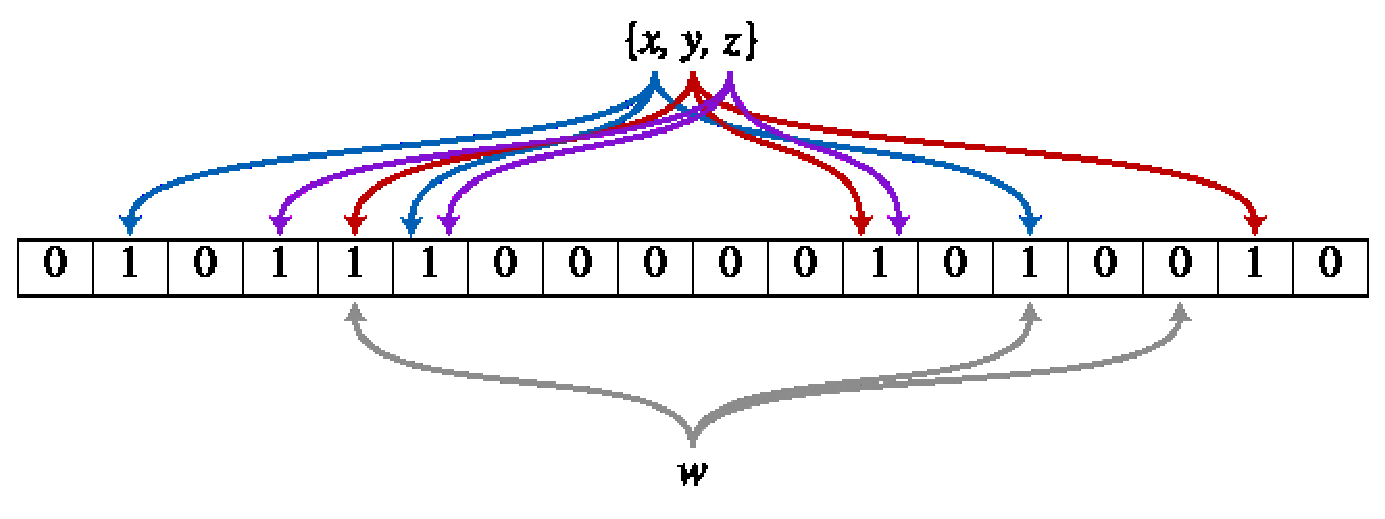
\includegraphics[keepaspectratio=true,width=.6\textwidth]{figures/muestra}
\end{figure}

Como poner una tabla:
\begin{center}
   \begin{tabular}{| c || c | c | c |}
      \hline
      	           & Load	& Store		& Total		\\ \hline \hline
	Accesses   & 105353	& 21423		& 126776	\\ \hline
	Hits       &  11644	&  1837		&  13481	\\ \hline
	Misses     &  93709 	& 19586		& 113295	\\ \hline
	Miss rate  & 88.95\%	& 91.43\%	& 89.37\%	\\ \hline
   \end{tabular}
\end{center}

Como poner c\'{o}digo:

\begin{lstlisting}[]
for( x = 0 ; x < grid_size ; x ++ ) {
  for( y = 0 ; y < grid_size ; y ++ ) {
    for( z = 0 ; z < grid_size ; z ++ ) {
      grid[gaddress(x,y,z,grid_size)] = ...
    }
  }
}
\end{lstlisting}

% vim: filetype=tex tw=75
